\documentclass[12pt]{ftec2101} 
% This template is modified from COLT 2020

% The following packages will be automatically loaded:
% amsmath, amssymb, natbib, graphicx, url, algorithm2e

\title{Course Project: Portfolio Optimization in Practice}
\usepackage{times}
\usepackage{amsmath}
\usepackage{hyperref}
\usepackage{enumitem}
\usepackage{graphicx}
\usepackage{float}
\usepackage{indentfirst}
\usepackage{booktabs}
\makeatletter
\def\set@curr@file#1{\def\@curr@file{#1}} %temp workaround for 2019 latex release
\makeatother
\usepackage[load-configurations=version-1]{siunitx} % newer version
%
% Use \Name{Author Name} to specify the name.
% If the surname contains spaces, enclose the surname
% in braces, e.g. \Name{John {Smith Jones}} similarly
% if the name has a "von" part, e.g \Name{Jane {de Winter}}.
% If the first letter in the forenames is a diacritic
% enclose the diacritic in braces, e.g. \Name{{\'E}louise Smith}

% Two authors with the same address
% \coltauthor{\Name{Author Name1} \Email{abc@sample.com}\and
%  \Name{Author Name2} \Email{xyz@sample.com}\\
%  \addr Address}

% Three or more authors with the same address:
% \coltauthor{\Name{Author Name1} \Email{an1@sample.com}\\
%  \Name{Author Name2} \Email{an2@sample.com}\\
%  \Name{Author Name3} \Email{an3@sample.com}\\
%  \addr Address}
\newcommand{\matr}[1]{\mathbf{#1}}
\newcommand{\vect}[1]{\mathbf{#1}}
% Authors with different addresses:
\coltauthor{%
 \Name{HU, Han} \Email{hanhu@link.cuhk.edu.hk}\\
 \addr Department of Information Engineering, CUHK
% \AND
% \Name{Author Name2} \Email{xyz@sample.com}\\ % uncomment this if you are working in a group of 2
% \addr Address 2%
}

\begin{document}

\maketitle


\section{Background and Introduction}
In this FTEC2101 course, multiple optimization methods are introduced and discussed during the class. These methods are not only beautiful theories, but also practical and powerful tools for solving real world problems. 


In this project, practical solutions for portfolio optimization using \textbf{Julia} are implemented on real-world dataset captured from stock market. The purpose of such optimization in portfolio design is to minimize the risk when pursuing the expected return within certain budget limitations. 


Different optimization methods are modelled and implemented in this project to investigate the optimal portfolio design. Here, the different methods have different performances and computational complexity when executing the task. It is also worth mention that finding the suitable optimization method with good performances and acceptable complexity for portfolio design is also an important task during practical implementation.

\section{Model and Theory}
\subsection{Task 1}
From the project specification, we first study the (simplified) Markowitz’s mean-variance Portfolio Optimization problem stated as
\begin{gather}
    \min_{\vect{p} \in \mathbb{R}^n} \quad \frac{1}{2}\vect{p}^T \boldsymbol{\Sigma} \vect{p}\\
    \textup{s.t.} \quad \vect{1}^T \vect{p} = B,\ \bar{\vect{r}}^T \vect{p} = R_d\ ,
    \label{Mark}
\end{gather}
where $B$ is the fixed budget, $R_d$ is the fixed desired return, and $\vect{1}$ is an all-one vector. The project specification also defines the covariance matrix $\boldsymbol{\Sigma}$ and the expected reward vector $\bar{\vect{r}}$ in detail.
\subsubsection{Subquestion (a)}
Derivation of the KKT conditions for the (simplified) Markowitz's mean-variance Portfolio Optimization problem stated in formula (\ref{Mark}) in project specification is:
\begin{align}
    L(p,\boldsymbol{\lambda}) = \frac{1}{2}\vect{p}^T\boldsymbol{\Sigma} \vect{p} + \lambda_{1} (\vect{1}^T \vect{p}-B) +\lambda_{2} (\bar{\vect{r}}^T \vect{p}-R_{d})\ ,
\end{align}
where $B$ is the fixed budget, $R_d$ is the fixed desired return and $\vect{1}$ is an all-one vector according to the project specification.


For the corvariance matrix, we have $\boldsymbol{\Sigma}^T = \boldsymbol{\Sigma}$. Then $\nabla \left(\frac{1}{2}\vect{p}^T \boldsymbol{\Sigma} \vect{p}\right) = \frac{1}{2}(\boldsymbol{\Sigma}\vect{p}+\boldsymbol{\Sigma}^T \vect{p}) = \boldsymbol{\Sigma}\vect{p}$. 


Solving the KKT condition, we have
\begin{align}
    \begin{cases}
        \nabla_{p} L(p,\boldsymbol{\lambda}) = 0 \\
        \nabla_{\lambda} L(p,\boldsymbol{\lambda}) = 0
    \end{cases}
    \implies
    \begin{cases}
        \boldsymbol{\Sigma}\vect{p}+\lambda_1 \vect{1} + \lambda_2 \bar{\vect{r}} = 0 \\
        \vect{1}^T \vect{p} - B = 0 \\
        \bar{\vect{r}}^T \vect{p} - R_d = 0
    \end{cases}
    \label{KKT:1}
\end{align}


From (\ref{KKT:1}), we can derive the optimal solution $\vect{p}^{*}$ as:
\begin{align}
    \begin{cases}
        \boldsymbol{p^{*}} = \boldsymbol{\Sigma}^{-1} \cdot (-\lambda_{1}^{*} \cdot \boldsymbol{1} - \lambda_{2}^{*}\cdot \boldsymbol{\bar{r}}) \\
        \lambda_{1}^{*} \cdot (\boldsymbol{1}^{T} \boldsymbol{\Sigma}^{-1} \boldsymbol{1}) + \lambda_{2}^{*} \cdot (\boldsymbol{1}^{T} \boldsymbol{\Sigma}^{-1} \boldsymbol{\bar{r}})=-B \\
        \lambda_{1}^{*} \cdot (\boldsymbol{\bar{r}}^{T} \boldsymbol{\Sigma}^{-1} \boldsymbol{1}) + \lambda_{2}^{*} \cdot (\boldsymbol{\bar{r}}^{T} \boldsymbol{\Sigma}^{-1} \boldsymbol{\bar{r}}) =-R_{d}
    \end{cases}
    \label{KKT:opt}
\end{align} 
Let
\begin{align}
    r_{0}=\boldsymbol{\bar{r}}^{T} \boldsymbol{\Sigma}^{-1} \boldsymbol{\bar{r}},~
    r_{1}=\boldsymbol{1}^{T} \boldsymbol{\Sigma}^{-1} \boldsymbol{\bar{r}},~
    r_{2}=\boldsymbol{1}^{T} \boldsymbol{\Sigma}^{-1} \boldsymbol{1}
    \label{R}
\end{align}
By plugging (\ref{R}) into (\ref{KKT:opt}), we obtain
\begin{align}
    \begin{cases}
        \lambda_{1}^{*} \cdot r_{2} + \lambda_{2}^{*} \cdot r_{1}=-B \\
        \lambda_{1}^{*} \cdot r_{1} + \lambda_{2}^{*} \cdot r_{0}=-R_{d}
    \end{cases}
    \label{KKT:opt:2}
\end{align}
Solving the equations in (\ref{KKT:opt:2}), we get  
\begin{align}
    \begin{cases}
        \lambda_1^* = \frac{r_1 R_d- r_0 B}{r_0 r_2 -r_1^2} \\
        \lambda_2^* = \frac{r_1 B - r_2 R_d}{r_0 r_2 -r_1^2}
    \end{cases}
\end{align}
Thus,
\begin{align}
    \vect{p}^* = \boldsymbol{\Sigma}^{-1} \cdot (-\lambda_{1}^{*} \cdot \boldsymbol{1} - \lambda_{2}^{*}\cdot \boldsymbol{\bar{r}}) =
    \frac{\boldsymbol{\Sigma}^{-1} \cdot \big \{  (r_{0}B-r_{1}R_{d})\boldsymbol{1} + (r_{2}R_{d}-r_{1}B)\boldsymbol{\bar{r}}   \big \}}{r_{0}r_{2}-r_{1}^{2}}
\end{align}
\subsubsection{Subquestion (b)}
From the simplified conditions given in the specification and calculations based on the additional conditions, we have 
\begin{align*}
    \bar{\vect{r}} =
    \begin{pmatrix}
        \bar{r}_1 \\
        1
    \end{pmatrix}\ ,
    r_0 = \bar{r}_1^2+1\ ,
    r_1 = \bar{r}_1 + 1\ , 
    r_2 = 2\ ,
    \boldsymbol{\Sigma} = \boldsymbol{\Sigma}^{-1} =
    \begin{pmatrix}
        1 & 0 \\
        0 & 1
    \end{pmatrix}
\end{align*}


Plug the above additional conditions into the given $\vect{p}^{*}$ given in subsection (a), we get
\begin{align}
    \vect{p}^{*} &= \frac{\boldsymbol{\Sigma}^{-1}\{[(\bar{r}_1^2+1)B-(\bar{r}_1+1)R_d]\vect{1}+[2R_d - (\bar{r}_1 + 1)B]\bar{\vect{r}}\}}{2\bar{r}_1^2 + 2 - (\bar{r}_1+1)^2} \\
    &= \frac{1}{\bar{r}_1 - 1} \cdot
    \begin{pmatrix}
        R_d - B \\
        B\bar{r}_1 - R_d
    \end{pmatrix}\\
    &=
    \begin{pmatrix}
        \frac{R_d-B}{\bar{r}_1 - 1} \\
        B+ \frac{B-R_d}{\bar{r}_1 - 1}
    \end{pmatrix}\ .
    \label{optimal:p}
\end{align}
By observing (\ref{optimal:p}), we can conclude that
\begin{enumerate}
    \item If $\bar{r}_1$ increases, since $R_d > B$, $p_1^{*}$ will decrease, $p_2^{*}$ will increase.
    \item If $R_d$ increases, $p_1^{*}$ will increase, $p_2^{*}$ will decrease.
\end{enumerate}

\subsection{Task 2}
In this part of the project, the framework is further extended with some realistic aspects of portfolio optimization. We further model the transaction amount and transaction cost. In task 2, a flat transaction cost of \$$c$ is incurred if we trade any share of stock $i$.


The mixed integer program formed is
\begin{gather}
    \min_{\vect{x}\in\mathbb{R}^n ,\  \vect{y}\in \mathbb{Z}^n} \quad (\vect{x}+\boldsymbol{\omega})^T \boldsymbol{\Sigma} (\vect{x}+\boldsymbol{\omega}) \\
    \label{mix:integer}
    \begin{aligned}
    \textup{s.t.} \quad \sum_{i=1}^{n} (x_i+\omega_i)\bar{r}_i \geq R_d\\
                \sum_{i=1}^{n} (x_i+y_i c) \leq B\\
                -M y_i \leq x_i \leq M y_i,\ i=1,\cdots,n\\
                x_i \geq -\omega_i,\ i = 1,\cdots,n\\
                y_i \in \{0,1\},\ i = 1,\cdots,n
\end{aligned}
\end{gather}
\subsection{Task 3}
In task 3, the transaction cost is modified to
\begin{align}
    \sum_{i=1}^n \phi(x_i) ,\ 
\end{align}
where $\phi(x_i) = ax_i^2$.
\subsubsection{Subquestion (a)}
The nonlinear program formed is 
\begin{gather}
    \min_{\vect{x} \in \mathbb{R}^{n}} \quad
    \quad (\vect{x}+\boldsymbol{\omega})^T \boldsymbol{\Sigma} (\vect{x}+\boldsymbol{\omega}) \\
\begin{aligned}
    \textup{s.t.} \quad \sum_{i=1}^{n} (x_i + \omega_i)\bar{r}_i \geq R_d \\
                        \sum_{i=1}^{n} (x_i + a x_i^2) \leq B \\
                        -M \leq x_i \leq M,\ i=1,\cdots,n \\
                        x_i \geq - \omega_{i - 1},\ i=1,\cdots,n
\end{aligned}
\label{nonlinear:p}
\end{gather}
\subsubsection{Subquestion (b)}
To write the nonlinear program as an SOCP, we first define a new vector $\vect{x'}$ as
\begin{align*}
    \vect{x'} = 
    \begin{pmatrix}
        t \\
        \vect{x}
    \end{pmatrix}\ , 
\end{align*}
where $\vect{x} \in \mathbb{R}^n$, $t \in \mathbb{R}$.
Then, the above nonlinear program can be written as:
\begin{gather}
    \min_{\vect{x'} \in \mathbb{R}^{n+1}} \quad
    \begin{pmatrix}
        1 \\
        0 \\
        \vdots \\
        0
    \end{pmatrix}^T
    \cdot \vect{x'}\\
\begin{aligned}
    \textup{s.t.} \quad \sum_{i=1}^{n} (x_i + \omega_i)\bar{r}_i \geq R_d \\
                        \sum_{i=1}^{n} (x_i + a x_i^2) \leq B \\
                        t \geq \sqrt{(\vect{x}+\boldsymbol{\omega})^T \boldsymbol{\Sigma} (\vect{x}+\boldsymbol{\omega})} \\
                        -M \leq x'_i \leq M,\ i=2,\cdots,n+1 \\
                        x'_i \geq - \omega_{i - 1},\ i=2,\cdots,n+1
\end{aligned}
\label{nonlinear:constraint}
\end{gather} 
We then need to modify the constraints in (\ref{nonlinear:constraint}) as
\begin{align}
    \sum_{i=1}^{n} (x_i + \omega_i)\bar{r}_i \geq R_d \implies \left \Vert 0 \vect{x'} + 
    \begin{pmatrix}
        R_d\\
        0\\
        \vdots\\
        0
    \end{pmatrix} \right \Vert \leq
    \begin{pmatrix}
        0\\
        \bar{\vect{r}}
    \end{pmatrix}^T \vect{x'} + \bar{\vect{r}}^T \boldsymbol{\omega}
\end{align}
\begin{align}
    \sum_{i=1}^{n} (x_i + a x_i^2) \leq B &\implies \sum_{i=1}^{n} \left(x_i + a x_i^2+\frac{1}{4a}\right) \leq B+\frac{n}{4a} \\
    &\implies \left \Vert \sqrt{a} \vect{x} + \frac{1}{2\sqrt{a}} \vect{1}\right \Vert \leq \sqrt{B+\frac{n}{4a}} \\
    &\implies \left \Vert 
    \begin{pmatrix}
        0 & \\
        \vdots & \sqrt{a} \matr{I} \\
        0 & 
    \end{pmatrix}\vect{x'} + \frac{1}{2\sqrt{a}} \cdot \vect{1} \right \Vert \leq 0 \cdot \vect{x'} + \sqrt{B+\frac{n}{4a}}
\end{align}
\begin{align}
    t \geq \sqrt{(\vect{x}+\boldsymbol{\omega})^T \boldsymbol{\Sigma} (\vect{x}+\boldsymbol{\omega})} &\implies \left \Vert \boldsymbol{\Sigma}^{\frac{1}{2}} \vect{x} + \boldsymbol{\Sigma}^{\frac{1}{2}}\boldsymbol{\omega}\right \Vert \leq t \\
    &\implies \left \Vert
    \begin{pmatrix}
        0 & \\
        \vdots & \boldsymbol{\Sigma}^{\frac{1}{2}}\\
        0 & 
    \end{pmatrix} \vect{x'} + \boldsymbol{\Sigma}^{\frac{1}{2}} \boldsymbol{\omega} \right \Vert \leq
    \begin{pmatrix}
        1 \\
        0 \\
        \vdots \\
        0
    \end{pmatrix}^T \vect{x'}
\end{align}
Thus, the formed SOCP is 
\begin{gather}
    \min_{\vect{x'} \in \mathbb{R}^{n+1}} \quad \begin{pmatrix}
        1 \\
        0 \\
        \vdots \\
        0
    \end{pmatrix}^T
    \cdot \vect{x'}\\
    \begin{aligned}
    \textup{s.t.} \quad  \left \Vert 0 \vect{x'} + 
    \begin{pmatrix}
        R_d\\
        0\\
        \vdots\\
        0
    \end{pmatrix} \right \Vert \leq
    \begin{pmatrix}
        0\\
        \bar{\vect{r}}
    \end{pmatrix}^T \vect{x'} + \bar{\vect{r}}^T \boldsymbol{\omega}\\
    \left \Vert 
    \begin{pmatrix}
        0 & \\
        \vdots & \sqrt{a} \matr{I} \\
        0 & 
    \end{pmatrix}\vect{x'} + \frac{1}{2\sqrt{a}} \cdot \vect{1} \right \Vert \leq 0 \cdot \vect{x'} + \sqrt{B+\frac{n}{4a}}\\
    \left \Vert
    \begin{pmatrix}
        0 & \\
        \vdots & \boldsymbol{\Sigma}^{\frac{1}{2}}\\
        0 & 
    \end{pmatrix} \vect{x'} + \boldsymbol{\Sigma}^{\frac{1}{2}} \boldsymbol{\omega} \right \Vert \leq
    \begin{pmatrix}
        1 \\
        0 \\
        \vdots \\
        0
    \end{pmatrix}^T \vect{x'}\\
    -M \leq x'_i \leq M,\ i=2,\cdots,n+1 \\
    x'_i \geq - \omega_{i - 1},\ i=2,\cdots,n+1
    \end{aligned}
\end{gather}
\section{Experiments}
In this section, we will focus on the details of the dataset, including its construction and information, the analysis of the dataset given by various formulations and the comparisons between the formulations.
\subsection{Task 4}
\begin{figure}[h]
    \centering
    \begin{minipage}{0.45\textwidth}
        \centering
        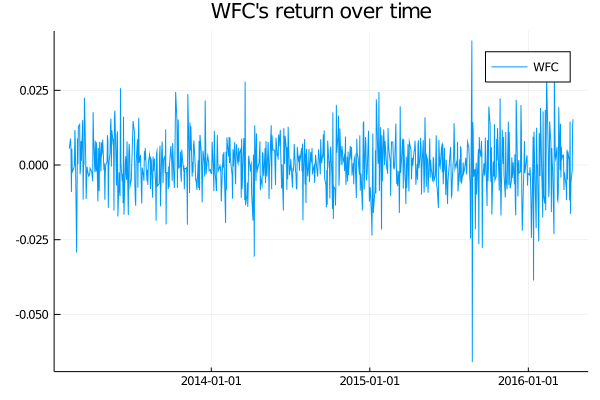
\includegraphics[scale=0.3]{stock1.png}
    \end{minipage}\hfill
    \begin{minipage}{0.45\textwidth}
        \centering
        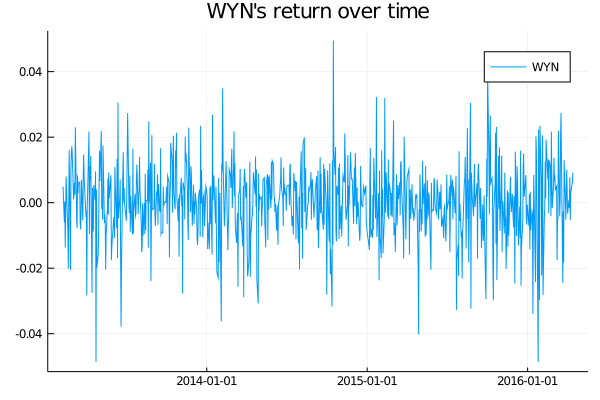
\includegraphics[scale=0.3]{stock2.png}
    \end{minipage}\vskip \baselineskip
    \begin{minipage}{0.45\textwidth}
        \centering
        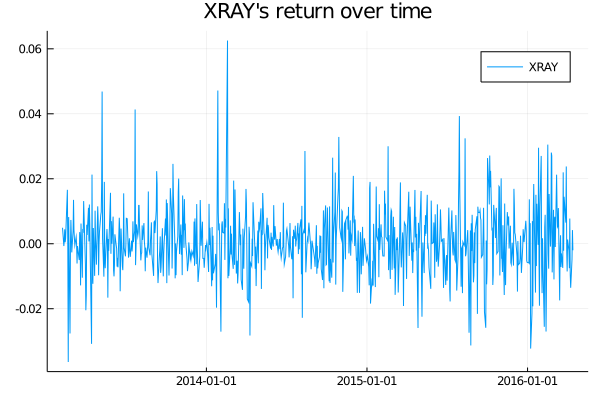
\includegraphics[scale=0.3]{stock3.png}
    \end{minipage}\hfill
    \begin{minipage}{0.45\textwidth}
        \centering
        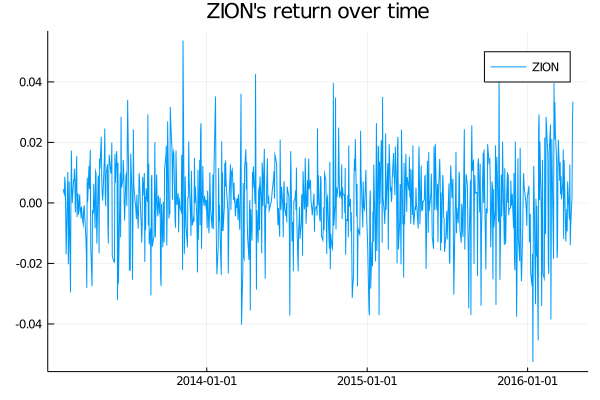
\includegraphics[scale=0.3]{stock4.png}
    \end{minipage}
    \caption{Return over time of selected stocks}
    \label{fig:stock}
\end{figure}

By directly observing the plotted return of the selected stocks as shown in Fig. \ref{fig:stock}, we can see that the x-axis represents the recorded time range of the selected stock, indicating the time range of the dataset is approximately from mid 2013 to early 2016, and the y-axis is the calculated return over time. We may notice that the this return value is calculated from daily change by using $\frac{\text{close~price-open~price}}{\text{open~price}}$. 
\subsection{Task 5}
\begin{figure}[htbp]
    \centering
    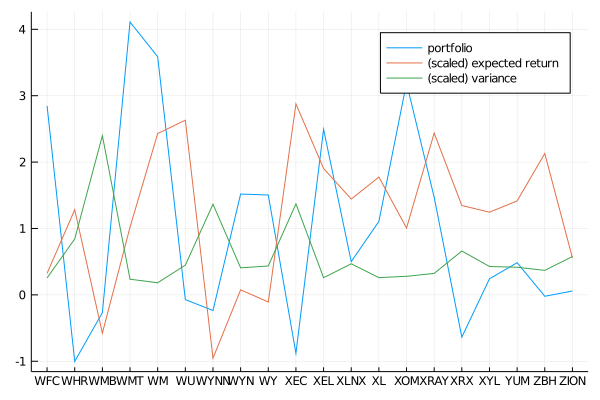
\includegraphics[scale=0.55]{5-normal.png}
    \caption{Portfolio found by deriving KKT conditions}
    \label{fig:KKT}
\end{figure}

From the result shown in Fig. \ref{fig:KKT}, we can observe that there are several negative terms in the portfolio found by this approach, which is not practical in real world cases. This indicates that more constraints are needed for accurate estimation and the current result may only serve as a reference in trend study.

The result shown in Fig. \ref{fig:KKT} also reveals the relationships behind the expected returns $\bar{r}_i$, the variance of each stock and the portfolio. The relationships can be summarized as:
\begin{itemize}
    \item The portfolio generally has positive correlation with the expected returns $\bar{r}_i$, while having negative correlation with the variance of each stock.
    \item The variance of each stock has more obvious affect on the portfolio than the expected returns as the portfolio is low at stocks with high variances regardless of what expected return it offered.
\end{itemize}
\begin{figure}[htbp]
    \centering
    \begin{minipage}{0.45\textwidth}
        \centering
        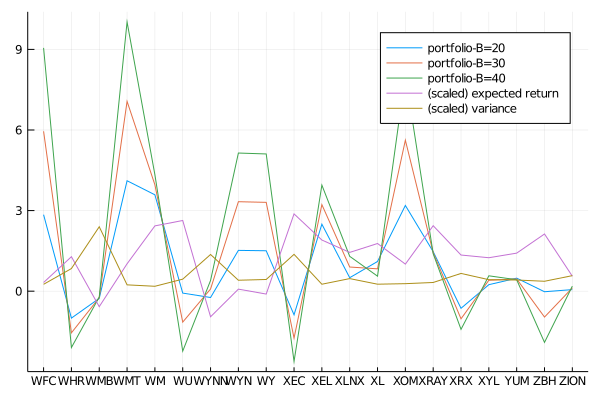
\includegraphics[scale=0.3]{5-exp-B.png}
        \caption{{\small Effects of budget on optimal portfolio}}
        \label{fig:B:eff}
    \end{minipage}\hfill
    \begin{minipage}{0.45\textwidth}
        \centering
        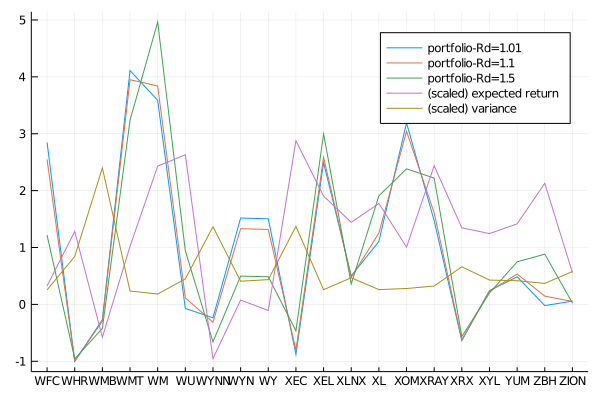
\includegraphics[scale=0.3]{5-exp-Rd.png}
        \caption{{\small Effects of desired return on optimal portfolio}}
        \label{fig:rd:eff}
    \end{minipage}
\end{figure}
To further investigate on the effects of desired return $R_d$ and budget $B$ on the optimal portfolio, we conducted experiments by trying different values for $B$ and $R_d$. The results are shown in Fig. \ref{fig:B:eff} and \ref{fig:rd:eff} and can be summarized as:
\begin{itemize}
    \item Increasing $B$ will introduce positive-correlated scale change in optimal portfolio without changing trend.
    \item Increasing $R_d$ will introduce positive-correlated impact factor change of the expected value to the optimal portfolio, which enhances the affect of the expected returns on the optimal portfolio.
\end{itemize}
\subsection{Task 6}
Here we present the results of the optimal portfolios found by three approaches in Fig. \ref{fig:three}.
\begin{figure}[htbp]
    \centering
    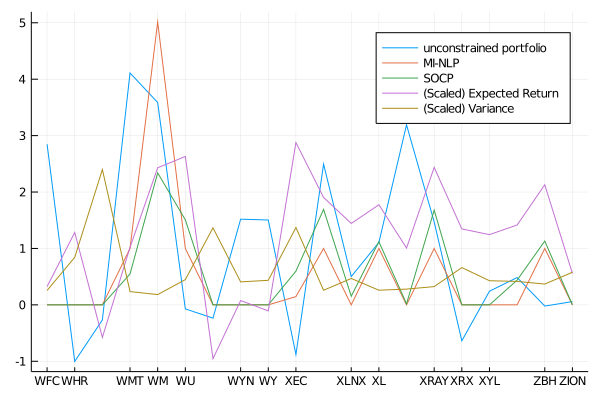
\includegraphics[scale=0.55]{three.png}
    \caption{Portfolio found by three approaches}
    \label{fig:three}
\end{figure}
From the figure, we can first conclude that the ML-NLP and SOCP approach fix the negative terms occurred in unconstrained portfolio. Meanwhile, the optimal portfolios found by three approaches share a similar pattern. Among the three approaches, the unconstrained portfolio seems to be most sensitive to the variance while other two approaches takes more expected return into consideration. For MI-NLP and SOCP, the former approach has a much more obvious max component than the latter one, while the latter approach has a more average distributed portfolio than the former one. 
\subsection{Task 7}
The intuitive performance comparison of the found optimal portfolios is given in Table \ref{table:result}.

From the table we can see that the MI-NLP formulation achieve the best balance between the total cost and Sharp ratio, but it achieves the lowest portfolio value. The SOCP formulation has low Sharp ratio, expected return and the same total cost as the unconstrained portfolio, though its portfolio value sits in the middle. The unconstrained portfolio has the best Sharp ratio, expected return and the portfolio value. However, considering it's having practically-impossible negative terms in the optimal portfolio, the real performance may be worse than the current calculated result.


\begin{table}
\centering
\begin{tabular}{ccccc}
\toprule  
Method&Sharp Ratio&Expected Return&Total Cost&Portfolio Value\\
\midrule  
MI-NLP&0.077430&0.0043659&28&11.161\\
SOCP&0.062327&0.0034452&40&11.227\\
Unconstrained&0.106874&0.0104528&40&20.000\\
\bottomrule 

\end{tabular}
\caption{Performance comparison of the portfolios}
\label{table:result}
\end{table}
\section{Competitive Task}
\section{Conclusion}
% It is a good habit to organize your reference in a bibliography (.bib) file. 
\bibliography{estr_bib}
 

\end{document}
